\documentclass{article}
\usepackage[utf8]{inputenc}
% are all of these packages really necessary?
% no.
% i'm just too lazy to only grab the packages i want for a specific
% document, so i just glob all of my most commonly used packages together
% this is bad practice.
\usepackage{amsmath,amsthm,amssymb,amsfonts, fancyhdr, color, comment, graphicx, environ, mdframed, soul, calc, enumitem, mdframed, xcolor, geometry, empheq, mathtools, tikz, pgfplots, caption, subcaption, hyperref}

\usetikzlibrary{external}
\tikzexternalize[prefix=tikz/,optimize command away=\includepdf]

%tikzpicture
\usepackage{tikz}
\usepackage{scalerel}
\usepackage{pict2e}
\usepackage{tkz-euclide}
\usetikzlibrary{calc}
\usetikzlibrary{patterns,arrows.meta}
\usetikzlibrary{shadows}
\usetikzlibrary{external}

%pgfplots
\usepackage{pgfplots}
\pgfplotsset{compat=newest}
\usepgfplotslibrary{statistics}
\usepgfplotslibrary{fillbetween}
\usepgfplotslibrary{polar}

\tikzset{external/export=true}
\pgfplotsset{
    standard/.style={
    axis line style = thick,
    trig format=rad,
    enlargelimits,
    axis x line=middle,
    axis y line=middle,
    enlarge x limits=0.15,
    enlarge y limits=0.15,
    every axis x label/.style={at={(current axis.right of origin)},anchor=north west},
    every axis y label/.style={at={(current axis.above origin)},anchor=south east}
    }
}
\newcommand*\widefbox[1]{\fbox{\hspace{2em}#1\hspace{2em}}}
% Command "alignedbox{}{}" for a box within an align environment
% Source: http://www.latex-community.org/forum/viewtopic.php?f=46&t=8144
\newlength\dlf  % Define a new measure, dlf
\newcommand\alignedbox[2]{
% Argument #1 = before & if there were no box (lhs)
% Argument #2 = after & if there were no box (rhs)
&  % Alignment sign of the line
{
\settowidth\dlf{$\displaystyle #1$}  
    % The width of \dlf is the width of the lhs, with a displaystyle font
\addtolength\dlf{\fboxsep+\fboxrule}  
    % Add to it the distance to the box, and the width of the line of the box
\hspace{-\dlf}  
    % Move everything dlf units to the left, so that & #1 #2 is aligned under #1 & #2
\boxed{#1 #2}
    % Put a box around lhs and rhs
}
}

\hypersetup{
    colorlinks=true,
    linkcolor=blue,
    filecolor=magenta,      
    urlcolor=cyan,
    pdftitle={Homework 6 Solutions},
    pdfpagemode=UseOutlines,
    bookmarksopen=true,
    pdfauthor={Christina Phan}
}
\newcommand{\lrp}[1]{\left( #1 \right)}
\newcommand{\abs}[1]{\left\vert #1 \right\vert}
\newcommand{\lra}[1]{\left\langle #1 \right\rangle}
\newcommand{\lrb}[1]{\left[ #1 \right]}
\newcommand{\iintR}[0]{\iint\limits_{R}}

\geometry{letterpaper, portrait, margin=1in}
\renewcommand{\footrulewidth}{0.8pt}
\setlength\parindent{0pt}
\pagestyle{fancy}
\lhead{Christina Phan}
\rhead{MAT 21D} 
\chead{\textbf{Homework 6 Solutions}}

\newcommand{\Solution}{\textit{Solution}}
\pgfplotsset{compat=1.18}
\begin{document}
\phantomsection
\addcontentsline{toc}{section}{Problem 1}\textbf{Problem 1}

Evaluate $\displaystyle \int_{-1}^1\int_0^{\sqrt{1-y^2}}\int_0^x x^2+y^2\,dz\,dx\,dy$ by converting to cylindrical coordinates.

\Solution

In cylindrical coordinates, our lower bound for $z$ is still $z=0$. Our upper bound for $z$ will be $z=r\cos\theta$ since in polar, $x=r\cos\theta$.

We can get our $r$ and $\theta$ by looking at the $xy$ region we're given. That is, graph $y=-1$, $y=1$, and $x=\sqrt{1-y^2}$.
\begin{center}
\resizebox{3cm}{!}{
    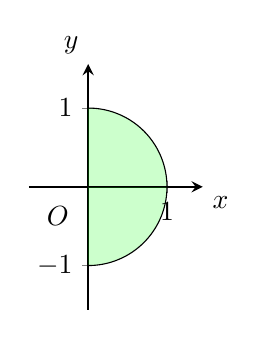
\begin{tikzpicture}
    \begin{axis}[standard,
            xtick={1},
            ytick={-1,1},
            samples=1000,
            xlabel={$x$},
            ylabel={$y$},
            xmin=-0.5,xmax=1.2,
            ymin=-1.2,ymax=1.2,
            x=1cm,
            y=1cm/1
           ]
\node[anchor=center,label=south west:$O$] at (axis cs:0,0){};
\addplot[name path=F,domain={0:1}]{sqrt(1-x^2)};
\addplot[name path=G,domain={0:1}]{-sqrt(1-x^2)};
\addplot[name path=H,domain={0:1}]{0};
\addplot[fill=green, fill opacity=0.2] fill between [of=F and H,soft clip={domain=0:1}];
\addplot[fill=green, fill opacity=0.2] fill between [of=G and H,soft clip={domain=0:1}];
    \end{axis}
    \end{tikzpicture}
}
\end{center}
From the graph, it looks like our $r$ is bounded below by $r=0$ and above by $r=1$. It also looks like our $\theta$ is bounded below by $-\dfrac{\pi}{2}$ and above by $\dfrac{\pi}{2}$.

Putting this all together, we get
\begin{align*}
    \int_{-1}^1\int_0^{\sqrt{1-y^2}}\int_0^x x^2+y^2\,dz\,dx\,dy&=\int_{-\frac{\pi}{2}}^{\frac{\pi}{2}}\int_0^1\int_0^{r\cos \theta}(r^2)r\,dz\,dr\,d\theta\\
    &=\int_{-\frac{\pi}{2}}^{\frac{\pi}{2}}\int_0^1\lrb{r^3z}_0^{r\cos\theta}\,dr\,d\theta\\
    &=\int_{-\frac{\pi}{2}}^{\frac{\pi}{2}}\int_0^1 r^4\cos\theta\,dr\,d\theta\\
    &=\int_{-\frac{\pi}{2}}^{\frac{\pi}{2}}\lrb{\frac{1}{5}r^5\cos\theta}_0^1\,d\theta\\
    &=\frac{1}{5}\cos\theta\,d\theta\\
    &=\lrb{\frac{1}{5}\sin\theta}_{-\frac{\pi}{2}}^{\frac{\pi}{2}}\\
    &=\lrp{\frac{1}{5}\sin \frac{\pi}{2}}-\lrp{\frac{1}{5}\sin -\frac{\pi}{2}}\\
    &=\frac{1}{5}-\lrp{-\frac{1}{5}}\\
    &=\boxed{\frac{2}{5}}
\end{align*}
\phantomsection
\addcontentsline{toc}{section}{Problem 2}\textbf{Problem 2}

Set up an integral to find the volume of the region:

\phantomsection
\addcontentsline{toc}{subsection}{2(a)}
\textbf{(a)} A right circular cylinder whose base is the circle $r=2\sin\theta$ in the $xy$-plane and whose top lies in the plane $z=4-y$.

\Solution

This fact that we want the volume of a \textit{cylinder} indicates to us that we should use \textit{cylindrical coordinates}.

Our lower bound for $z$ is $z=0$ and our upper bound for $z$ is $z=4-y$. In terms of $r$ and $\theta$, our upper bound for $z$ is $z=4-r\sin\theta$.

Since our base is the circle $r=2\sin\theta$, we know that this is a one petal polar graph with $r$ going from $0$ to $r=2\sin\theta$ and $\theta$ going from $0$ to $\pi$. You can graph this curve by hand, or on Desmos to confirm.

Putting these bounds all together, we get
\begin{equation*}
    \boxed{V=\int_0^\pi\int_0^{2\sin\theta}\int_0^{4-r\sin\theta}r\,dz\,dr\,d\theta}
\end{equation*}
\phantomsection
\addcontentsline{toc}{subsection}{2(b)}\textbf{(b)} The region bounded below by the cone $z=\sqrt{x^2+y^2}$ and above by the plane $z = 1$ (use spherical coordinates).

\Solution

Our lower bound for $\rho$ is $\rho =0$. We can get our upper bound for $\rho$ from the plane $z=1$. If $z=1$, then $\rho \cos \phi=1\implies \rho = \sec\phi$.

Our lower bound for $\phi$ is $0$. We can get our upper bound for $\phi$ from the cone $z=\sqrt{x^2+y^2}$. If $z=\sqrt{x^2+y^2}$, then $z=\sqrt{r^2}=r$ If $z=r$, then $\tan \phi = \dfrac{r}{z}=1\implies\phi =\dfrac{\pi}{4}$.

Since we're taking the region of the whole cone area, we're fully rotating over the $z$-axis, so our $\theta$ goes from $0$ to $2\pi$.

Putting this all together, we get
\begin{align*}
   \boxed{ V=\int_0^{2\pi}\int_0^{\pi/4}\int_0^{\sec \phi} \rho^2 \sin\phi \, d\rho\,d\phi\,d\theta}
\end{align*}
\phantomsection
\addcontentsline{toc}{subsection}{2(c)}\textbf{(c)} The sphere $\rho =2$ (use all three coordinate systems).

\Solution

\phantomsection
\addcontentsline{toc}{subsubsection}{Cartesian Coordinates}\textbf{Cartesian Coordinates}

If $\rho=2$, then $x^2+y^2+z^2=2^2=4$. In terms of $x$ and $y$, our $z$ is bounded below by $z=-\sqrt{4-x^2+y^2}$ and above by $z=\sqrt{4-x^2+y^2}$.

Setting $z=0$ for our top view, we get $x^2+y^2+0^2=4$. In terms of $x$, our $y$ is bounded below by $y=-\sqrt{4-x^2}$ and above by $y=\sqrt{4-x^2}$.

Setting $z=0$ and $y=0$ for our $x$ bounds, we get $x^2+0^2+0^2=4$. Our $x$ is bounded below by $x=-{2}$ and above by $x={2}$.

Putting this all together, we get
\begin{equation*}
    V=\int_{-{2}}^{{2}}\int_{-\sqrt{4-x^2}}^{\sqrt{4-x^2}}\int_{-\sqrt{4-x^2+y^2}}^{\sqrt{4-x^2+y^2}}\,dz\,dy\,dx
\end{equation*}
\phantomsection
\addcontentsline{toc}{subsubsection}{Cylindrical Coordinates}\textbf{Cylindrical Coordinates}

If $\rho=2$, then $x^2+y^2+z^2=2^2=4$. In terms of $x$ and $y$, our $z$ is bounded below by $z=-\sqrt{4-x^2+y^2}$ and above by $z=\sqrt{4-x^2+y^2}$.

In polar, $x^2+y^2=r^2$, so our lower bound for $z$ is $z=-\sqrt{4-r^2}$ and our upper bound for $z$ is $z=\sqrt{4-r^2}$.

Setting $z=0$ for our top view, we get $x^2+y^2+0^2=4$ which translates to $r^2=4$ in polar. Our lower bound for $r$ is $0$ and our upper bound for $r$ is $2$.

Since our top view is the circle $r=2$, our $\theta$ goes from $0$ to $2\pi$.

Putting this all together, we get
\begin{equation*}
    V=\int_0^{2\pi}\int_0^2\int_{-\sqrt{4-r^2}}^{\sqrt{4-r^2}}r\,dz\,dr\,d\theta
\end{equation*}
\phantomsection
\addcontentsline{toc}{subsubsection}{Spherical Coordinates}\textbf{Spherical Coordinates}

If $\rho=2$, then our lower bound for $\rho$ is $\rho=0$ and our upper bound for $\rho$ is $\rho =2$.

Since this is a sphere, our $\phi$ will go from the ``north pole" to the ``south pole". That is, our $\phi$ will go from $0$ to $\pi$.

Since this is a sphere, our $\theta$ will go around the entire $z$-axis. That is, our $\theta$ will go from $0$ to $2\pi$.

Putting this all together, we get
\begin{equation*}
    V=\int_0^{2\pi}\int_0^{\pi}\int_0^2 \rho^2\sin\phi\,d\rho\,d\phi\,d\theta
\end{equation*}
Our final answer is
\begin{subequations}
    \begin{empheq}[box=\widefbox]{align}
        \text{Cartesian: }&V=\int_{-{2}}^{{2}}\int_{-\sqrt{4-x^2}}^{\sqrt{4-x^2}}\int_{-\sqrt{4-x^2+y^2}}^{\sqrt{4-x^2+y^2}}\,dz\,dy\,dx\nonumber\\
        \text{Cylindrical: }&V=\int_0^{2\pi}\int_0^2\int_{-\sqrt{4-r^2}}^{\sqrt{4-r^2}}r\,dz\,dr\,d\theta\nonumber\\
        \text{Spherical: }&V=\int_0^{2\pi}\int_0^{\pi}\int_0^2 \rho^2\sin\phi\,d\rho\,d\phi\,d\theta\nonumber
    \end{empheq}
\end{subequations}
\phantomsection
\addcontentsline{toc}{section}{Problem 3}\textbf{Problem 3}

Find the volume of the region:

\phantomsection
\addcontentsline{toc}{subsection}{3(a)}\textbf{(a)} The region in the first octant bounded below by the cone $\phi =\dfrac{\pi}{4}$ and above by
the sphere $\rho = 3$.

\Solution

The \textit{cone} keyword $\phi$, and $\rho$ in the problem indicates that this volume should be set up using spherical coordinates.

Our $\rho$ is bounded below by $\rho = 0$ and above by $\rho = 3$.

Our $\phi$ is bounded below by $\phi = 0$ and above by $\phi = \dfrac{\pi}{4}$.

Since we are going around the first octant, our $\theta$ is bounded below by $\theta=0$ and above by $\theta=\dfrac{\pi}{2}$.

Putting this all together, we get
\begin{align*}
    V&=\int_0^{{\pi}/{2}}\int_0^{{\pi}/{4}}\int_0^3\rho^2\sin\phi\,d\rho\,d\phi\,d\theta\\
    &=\int_0^{{\pi}/{2}}\int_0^{{\pi}/{4}}\lrb{\frac{1}{3}\rho^3\sin\phi}_0^3\,d\phi\,d\theta\\
    &=\int_0^{{\pi}/{2}}\int_0^{{\pi}/{4}} 9\sin\phi\,d\phi\,d\theta\\
    &=\int_0^{{\pi}/{2}} \lrb{-9\cos\theta}_0^{\pi/4}\,d\theta\\
    &=\int_0^{{\pi}/{2}} -\frac{9}{\sqrt{2}}+9\,d\theta\\
    &=\lrb{-\frac{9}{\sqrt{2}}\theta+9\theta}_0^{\pi/2}\\
    &=\boxed{-\frac{9}{2\sqrt{2}}\pi+\frac{9}{2}\pi}
\end{align*}
\phantomsection
\addcontentsline{toc}{subsection}{3(b)}\textbf{(b)} The region cut from the sphere $\rho \leq a$ by the half-planes $\theta = 0$ and $\theta = \dfrac{\pi}{6}$ in the first octant.

\Solution

The \textit{sphere} keyword and $\phi$ in the problem indicates that this volume should be set up using spherical coordinates.

Our $\rho$ is bounded below by $\rho = 0$ and above by $\rho = a$.

Since our region is a sphere in the first octant, our $\phi$ is bounded below by $\phi = 0$ and above by $\phi = \dfrac{\pi}{2}$ (we go from the ``north" pole to the middle $z=0$ plane, a right angle).

As specified in the problem, our $\theta$ is bounded below by $\theta = 0$ and $\theta = \dfrac{\pi}{6}$.

Putting this all together, we get
\begin{align*}
    V&=\int_0^{\pi/6}\int_0^{\pi/2}\int_0^{a}\rho^2\sin\phi\,d\rho\,d\phi\,d\theta\\
    &=\int_0^{\pi/6}\int_0^{\pi/2} \lrb{\frac{1}{3}\rho^3 \sin\phi}_0^a\,d\phi \,d\theta\\
    &=\int_0^{\pi/6}\int_0^{\pi/2} \frac{1}{3}a^3\sin\phi\,d\phi\,d\theta\\
    &=\int_0^{\pi/6}\lrb{-\frac{1}{3}a^3\cos\phi}_0^{\pi/2}\,d\theta\\
    &=\int_0^{\pi/6} \frac{1}{3}a^3\,d\theta\\
    &=\lrb{\frac{1}{3}a^3\theta}_0^{\pi/6}\\
    &=\boxed{\frac{1}{18}a^3\pi}
\end{align*}
\phantomsection
\addcontentsline{toc}{subsection}{3(c)}\textbf{(c)} The smaller region cut from the sphere $\rho \leq 2$ by the plane $z=1$.

\Solution

The \textit{sphere} keyword and $\rho$ indicates that this volume should be set up using spherical coordinates.

Our $\rho$ is bounded above by $\rho = 2$. We can get our lower bound of $\rho $ from the plane $z=1$. Since $z=1$, in spherical coordinates, $r\cos\phi = 1\implies r=\sec \phi$.

Let's graph the sphere $x^2+y^2+z^2=2^2$ and the plane $z=1$ on from a front view. Our sphere becomes a circle of radius $2$ and our $z=1$ is just a line. 
You'll notice how we get $\phi$ below. The angle $\phi$ can be obtained from $\cos \phi = \dfrac{1}{2}\implies \phi =\dfrac{\pi}{3}$.
\begin{center}
\resizebox{3.5cm}{!}{


\tikzset{every picture/.style={line width=0.75pt}} %set default line width to 0.75pt        

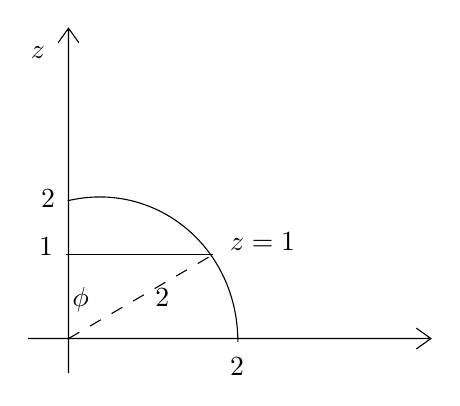
\begin{tikzpicture}[x=0.75pt,y=0.75pt,yscale=-1,xscale=1]
%uncomment if require: \path (0,300); %set diagram left start at 0, and has height of 300

%Shape: Axis 2D [id:dp43042752003169704] 
\draw  (181,214.51) -- (375,214.51)(200.4,65) -- (200.4,231.12) (368,209.51) -- (375,214.51) -- (368,219.51) (195.4,72) -- (200.4,65) -- (205.4,72)  ;
%Curve Lines [id:da7010778859227402] 
\draw    (200,148.12) .. controls (242,138.12) and (282,170.12) .. (282,216.12) ;
%Straight Lines [id:da97768980383442] 
\draw    (199,174.12) -- (270,174.12) ;
%Straight Lines [id:da9543514175258525] 
\draw  [dash pattern={on 4.5pt off 4.5pt}]  (200.4,214.51) -- (270,174.12) ;

% Text Node
\draw (277,162.4) node [anchor=north west][inner sep=0.75pt]    {$z=1$};
% Text Node
\draw (181,72.4) node [anchor=north west][inner sep=0.75pt]    {$z$};
% Text Node
\draw (186,141.4) node [anchor=north west][inner sep=0.75pt]    {$2$};
% Text Node
\draw (277,222.4) node [anchor=north west][inner sep=0.75pt]    {$2$};
% Text Node
\draw (201,188.4) node [anchor=north west][inner sep=0.75pt]    {$\phi $};
% Text Node
\draw (185,164.4) node [anchor=north west][inner sep=0.75pt]    {$1$};
% Text Node
\draw (241,189.4) node [anchor=north west][inner sep=0.75pt]    {$2$};


\end{tikzpicture}

}
\end{center}

Our $\phi$ is bounded below by $\phi=0$ and above by $\phi = \dfrac{\pi}{3}$.

Since this is a sphere-ish, our $\theta$ will go around the entire $z$-axis. That is, our $\theta$ is bounded below by $\theta=0$ and above by $\theta =2\pi$.

Putting this all together, we get
\begin{align*}
    V&=\int_0^{2\pi}\int_0^{\pi/3}\int_{\sec\phi}^2\rho^2\sin\phi\,d\rho\,d\phi\,d\theta\\
    &=\int_0^{2\pi}\int_0^{\pi/3}\lrb{\frac{1}{3}\rho^3\sin\phi}_{\sec\phi}^2\,d\phi\,d\theta\\
    &=\int_0^{2\pi}\int_0^{\pi/3} \frac{8}{3}\sin\phi -\frac{1}{3}\sec^3\phi\sin\phi\,d\phi\,d\theta\\
    &=\int_0^{2\pi}\int_0^{\pi/3} \frac{8}{3}\sin\phi- \frac{1}{3}\sec^2\phi \tan\phi \,d\phi\,d\theta\tag{$\displaystyle \sec^3\phi\sin\phi=\frac{1}{\cos^3\phi}\sin\phi=\frac{1}{\cos^2\phi}\frac{\sin\phi}\cdot{\cos\phi}$}\\
    &=\int_0^{2\pi}\lrb{-\frac{8}{3}\cos\phi-\frac{1}{6}\tan^2\phi}_0^{\pi/3}\,d\theta\tag{you can also $u$ sub}\\
    &=\int_0^{2\pi} \lrp{-\frac{8}{3}\lrp{\frac{1}{2}}-\frac{1}{6}\lrp{\sqrt{3}}^2}-\lrp{-\frac{8}{3}-0}\,d\theta\\
    &=\int_0^{2\pi} -\frac{4}{3}-\frac{1}{2}+\frac{8}{3}\,d\theta\\
    &=\lrb{-\frac{4}{3}\theta -\frac{1}{2}\theta+\frac{8}{3}\theta}_0^{2\pi}\\
    &=-\frac{8}{3}\pi - \pi + \frac{16}{3}\pi\\
    &=\boxed{\frac{5}{3}\pi}
\end{align*}

\phantomsection
\addcontentsline{toc}{subsection}{3(d)}\textbf{(d)} The region cut form the ''thick-walled" cylinder $1\leq x^2+y^2\leq 2$ by the cones $z=\sqrt{x^2+y^2}$ and $z=-\sqrt{x^2+y^2}$.

\Solution

Trust me when I say that this looks like a job for cylindrical coordinates, not spherical coordinates. The \textit{cylinder} keyword and lack of $\rho$ and $\phi$ in the problem deters me from using spherical coordinates here.

Our $z$ is bounded below by $z=-\sqrt{x^2+y^2}$ and above by $z=\sqrt{x^2+y^2}$. In terms of $r$, our $z$ bounded below by $z=-\sqrt{r^2}=-r$ and above by $z=\sqrt{r^2}=r$ since $x^2+y^2=r^2$.

From the problem, $1\leq x^2+y^2\leq 2$ which is $1\leq r^2\leq 2$ in polar since $x^2+y^2=r^2$. Therefore, our $r$ is bounded below by $r=1$ and above by $r=\sqrt{2}$.

Since we are going around the entire $z$-axis for the cylinder, our $\theta$ is bounded below by $\theta=0$ and above by $\theta=2\pi$.

Putting this all together, we get
\begin{align*}
    \int_0^{2\pi}\int_1^{\sqrt{2}}\int_{-r}^{r}r\,dz\,dr\,d\theta&= \int_0^{2\pi}\int_1^{\sqrt{2}}\lrb{rz}_{-r}^r\,dr\,d\theta\\
    &=\int_0^{2\pi}\int_1^{\sqrt{2}} r^2 -( -r^2)\,dr\,d\theta\\
     &=\int_0^{2\pi}\int_1^{\sqrt{2}}  2r^2\,dr\,d\theta\\
     &=\int_0^{2\pi}\lrb{\frac{2}{3}r^3}_1^{\sqrt{2}}\,d\theta\\
     &=\int_0^{2\pi} \frac{4\sqrt{2}}{3}-\frac{2}{3}\,d\theta\\
     &=\lrb{\frac{4\sqrt{2}}{3}\theta-\frac{2}{3}\theta}_0^{2\pi}\\
     &=\frac{4\sqrt{2}}{3}(2\pi)-\frac{2}{3}(2\pi)\\
     &=\boxed{\frac{8\pi\sqrt{2}-4\pi}{3}}
\end{align*}
\phantomsection
\addcontentsline{toc}{subsection}{3(e)}\textbf{(e)} The region inside the sphere $x^2+y^2+z^2=2$ and outside the cylinder $x^2+y^2=1$.

\Solution

Trust me when I say that this looks like a job for cylindrical coordinates, not spherical coordinates. The \textit{cylinder} keyword and lack of $\rho$ and $\phi$ in the problem deters me from using spherical coordinates here.

We can get our upper and lower bounds for $z$ from the sphere $x^2+y^2+z^2=2$ (the cylinder is \textit{inside} the sphere, so it's $z$ values are irrelevant). Our upper and lower bounds for $z$ are $z=\pm\sqrt{2-x^2-y^2}$. In polar, our upper and lower bounds for $z$ are $z=\pm\sqrt{2-r^2}$ since $x^2+y^2=r^2$.

If we look at the region from a top view by setting $z=0$, we can get our bounds for $r$ and $\theta$. Our lower $r$ is bounded below by the cylinder $x^2+y^2=1$ and above by the circle $x^2+y^2+0^2=2$. In polar, our lower bound for $r$ is $r=1$ and our upper bound for $r$ is $r=\sqrt{2}$ since $x^2+y^2=r^2$.

Again, from the top view, we can see that our region is the full circle. Therefore, our lower bound for $\theta$ is $\theta=0$ and our upper bound for $\theta$ is $\theta=2\pi$.

Putting this all together, we get
\begin{align*}
    V&=\int_0^{2\pi}\int_1^{\sqrt{2}}\int_{-\sqrt{2-r^2}}^{\sqrt{2-r^2}}r\,dz\,dr\,d\theta\\
    &=\int_0^{2\pi}\int_1^{\sqrt{2}}\lrb{rz}_{-\sqrt{2-r^2}}^{\sqrt{2-r^2}}\,dr\,d\theta\\
    &=\int_0^{2\pi}\int_1^{\sqrt{2}} r\sqrt{2-r^2}-(-r\sqrt{2-r^2})\,dr\,d\theta\\
    &=\int_0^{2\pi}\int_1^{\sqrt{2}} 2r\sqrt{2-r^2}\,dr\,d\theta\\
    &u=2-r^2 \hspace{2em} du=-2r\,dr\\
    &u(1)=1\hspace{2em}u(\sqrt{2})=0\\
    &=\int_0^{2\pi}\int_1^0 -\sqrt{u}\,du\,d\theta\\
    &=\int_0^{2\pi}\int_0^1 \sqrt{u}\,du\,d\theta\\
    &=\int_0^{2\pi}\lrb{\frac{2}{3}u^{3/2}}_0^1\,d\theta\\
    &=\int_0^{2\pi}\frac{2}{3}\,d\theta\\
    &=\lrb{\frac{2}{3}\theta}_0^{2\pi}\\
    &=\boxed{\frac{4}{3}\pi}
\end{align*}

\phantomsection
\addcontentsline{toc}{subsection}{3(f)}\textbf{(f)} The region bounded above by the sphere $x^2 + y^2 + z^2 = 2$ and below by the paraboloid $z = x^2 + y^2$.

\Solution

Trust me when I say that this looks like a job for cylindrical coordinates, not spherical coordinates. The lack of $\rho$ and $\phi$ in the problem deters me from using spherical coordinates here.

Our lower bound for $z$ is given by the paraboloid $z=x^2+y^2$. Our upper bound for $z$ is given by the sphere $x^2+y^2+z^2=2$ which is $z=\sqrt{2-x^2-y^2}$. In polar, our lower bound for $z$ is $z=r^2$ and our upper bound for $z$ is $z=\sqrt{2-r^2}$ since $x^2+y^2=r^2$.

Our bounds for $r$ and $\theta$ can be given by looking at a top view of the region. We can get our top view from the intersection of $z=x^2+y^2$ and $x^2+y^2+z^2=2$.
\begin{align*}
    z+z^2&=2\\
    z^2+z-2&=0\\
    (z+2)(z-1)&=0\\
    z&=1\tag{only positive $z$!}
\end{align*}
Since at the intersection $z=1$, $1=x^2+y^2$ at our top view. This is a filled-in circle with radius $r=1$ going from $0$ to $2\pi$.

Putting this all together, we get
\begin{align*}
    V&=\int_0^{2\pi}\int_0^1\int_{r^2}^{\sqrt{2-r^2}}r\,dz\,dr\,d\theta\\
    &=\int_0^{2\pi}\int_0^1\lrb{rz}_{r^2}^{\sqrt{2-r^2}}\,dr\,d\theta\\
    &=\int_0^{2\pi}\int_0^1 r\sqrt{2-r^2}-r^3\,dr\,d\theta\\
    &=\int_0^{2\pi}\lrb{-\frac{1}{3}(2-r^2)^{3/2}-\frac{1}{4}r^4}_0^1\,d\theta\tag{you can also do a $u$ sub}\\
    &=\int_0^{2\pi} \lrp{-\frac{1}{3}-\frac{1}{4}}-\lrp{-\frac{1}{3}(2)^{3/2}-0}\,d\theta\\
    &=\int_0^{2\pi} \frac{2\sqrt{2}-1}{3}-\frac{1}{4}\,d\theta\\
    &=\lrb{\frac{2\sqrt{2}-1}{3}\theta -\frac{1}{4}\theta}_0^{2\pi}\\
    &=\boxed{\frac{4\sqrt{2}-2}{3}\pi-\frac{1}{2}\pi}
\end{align*}
\phantomsection
\addcontentsline{toc}{section}{Problem 4}\textbf{Problem 4} 

What symmetry does a surface given in spherical coordinates by $\rho =f(\phi)$ have?

\Solution

If $\rho=f(\phi)$, then in spherical coordinates we have $\big(f(\phi),\phi,\theta)$. 

Since $\theta$ is pretty much a ``free variable", then $\big(f(\phi),\phi,\theta)=\big(f(\phi),\phi,\theta+\pi)$. Graphically, this makes sense. We can rotate $\rho = f(\phi)$ along the $z$-axis and produce the same region because the angle $\theta$ will not affect $\rho$.

Therefore, there is symmetry with respect to the $z$-axis.
\qed

\textbf{Problem}

Let's have $(0,0,3)$ be our base point for no particular reason.
\begin{align*}
    \mathbf{u}&=\lra{0-1,0-0,3-0}=\lra{-1,0,3}\\
    \mathbf{v}&=\lra{0-0,0-2,3-0}=\lra{0,-2,3}\\
    \mathbf{u}\times\mathbf{v}&=\begin{vmatrix}
\mathbf{i} & \mathbf{j} & \mathbf{k}\\
-1 & 0 & 3\\
0 & -2 & 3\\
\end{vmatrix}\\
&=\begin{vmatrix}
0 & 3\\
-2 & 3\\
\end{vmatrix}\mathbf{i}-
\begin{vmatrix}
-1 & 3\\
0 & 3\\
\end{vmatrix}\mathbf{j}+
\begin{vmatrix}
-1 & 0\\
0 & -2\\
\end{vmatrix}\mathbf{k}\\
&=\big(\left(0\right)\left(3\right)-\left(3\right)\left(-2\right)\big)\mathbf{i}-\big(\left(-1\right)\left(3\right)-\left(3\right)\left(0\right)\big)\mathbf{j}+\big(\left(-1\right)\left(-2\right)-\left(0\right)\left(0\right)\big)\mathbf{k}\\
&= 6\mathbf{i}+3\mathbf{j}+2\mathbf{k}\\
&=\lra{6,3,2}
\end{align*}
Recall that a plane can be represented as 
\begin{align*}
    a(x-x_0)+b(y-y_0)+c(z-z_0)=0
\end{align*}
Using $(0,0,3)$ as our base point and $\mathbf{u}\times\mathbf{v}=\lra{6,3,2}$ as our $a$, $b$, and $c$ values,
\begin{align*}
    6(x-0)+3(y-0)+2(z-3)&=0\\
    6x+3y+2z-6&=0\\
    2z&=6-6x-3y\\
    z&=3-3x-\frac{3}{2}y
\end{align*}
\end{document}
